\documentclass[11pt, twocolumn, a4paper]{article}
\usepackage[margin=0.5in]{geometry}
\usepackage{graphicx}
\usepackage{multicol}
\usepackage{subfig}
\pagenumbering{arabic}

\title{\textbf{Landmarks automatic identification by structure analysis}}
\author{Marie \textbf{BEURTON-AIMAR} \\  LaBRI - University of Bordeaux,
			\\ Bordeaux - France \\ \texttt{marie.beurton@labri.fr}		
		\and \textbf{LE} Van Linh \\ ITDLU - University of Dalat,
		\\ Dalat - Vietnam \\ 	\texttt{linhlv@dlu.edu.vn}
	}  
\date{}
\begin{document}

\twocolumn[
	\begin{@twocolumnfalse}
\maketitle
\begin{abstract}

Landmarks are points on the object which we can use it to identify or classify the objects. In this paper, we present a method to identify the landmarks automatically on the parts of beetle images and evaluate the results by statistic method. Based on the results, we will decide to replace the manual landmarks by automatic landmarks on beetle images. This method implemented from the article \textbf{"Automatic identification of landmarks in digital images"}\cite{palaniswamy2010automatic}.
\end{abstract}

\textbf{\textit{Keywords}:} Landmarks identification, image processing	
	\end{@twocolumnfalse}~\\
]
\section{Introduction}
Landmarks are points that can be defined in all specimens and located precisely. They are widely used in many biological and medical applications. Besides, the landmarks can be used to classify the objects into the groups by characteristic of the landmarks on objects. 
\begin{figure}[h!]
\centering
\subfloat[Right mandible]
{\label{fig:example_111}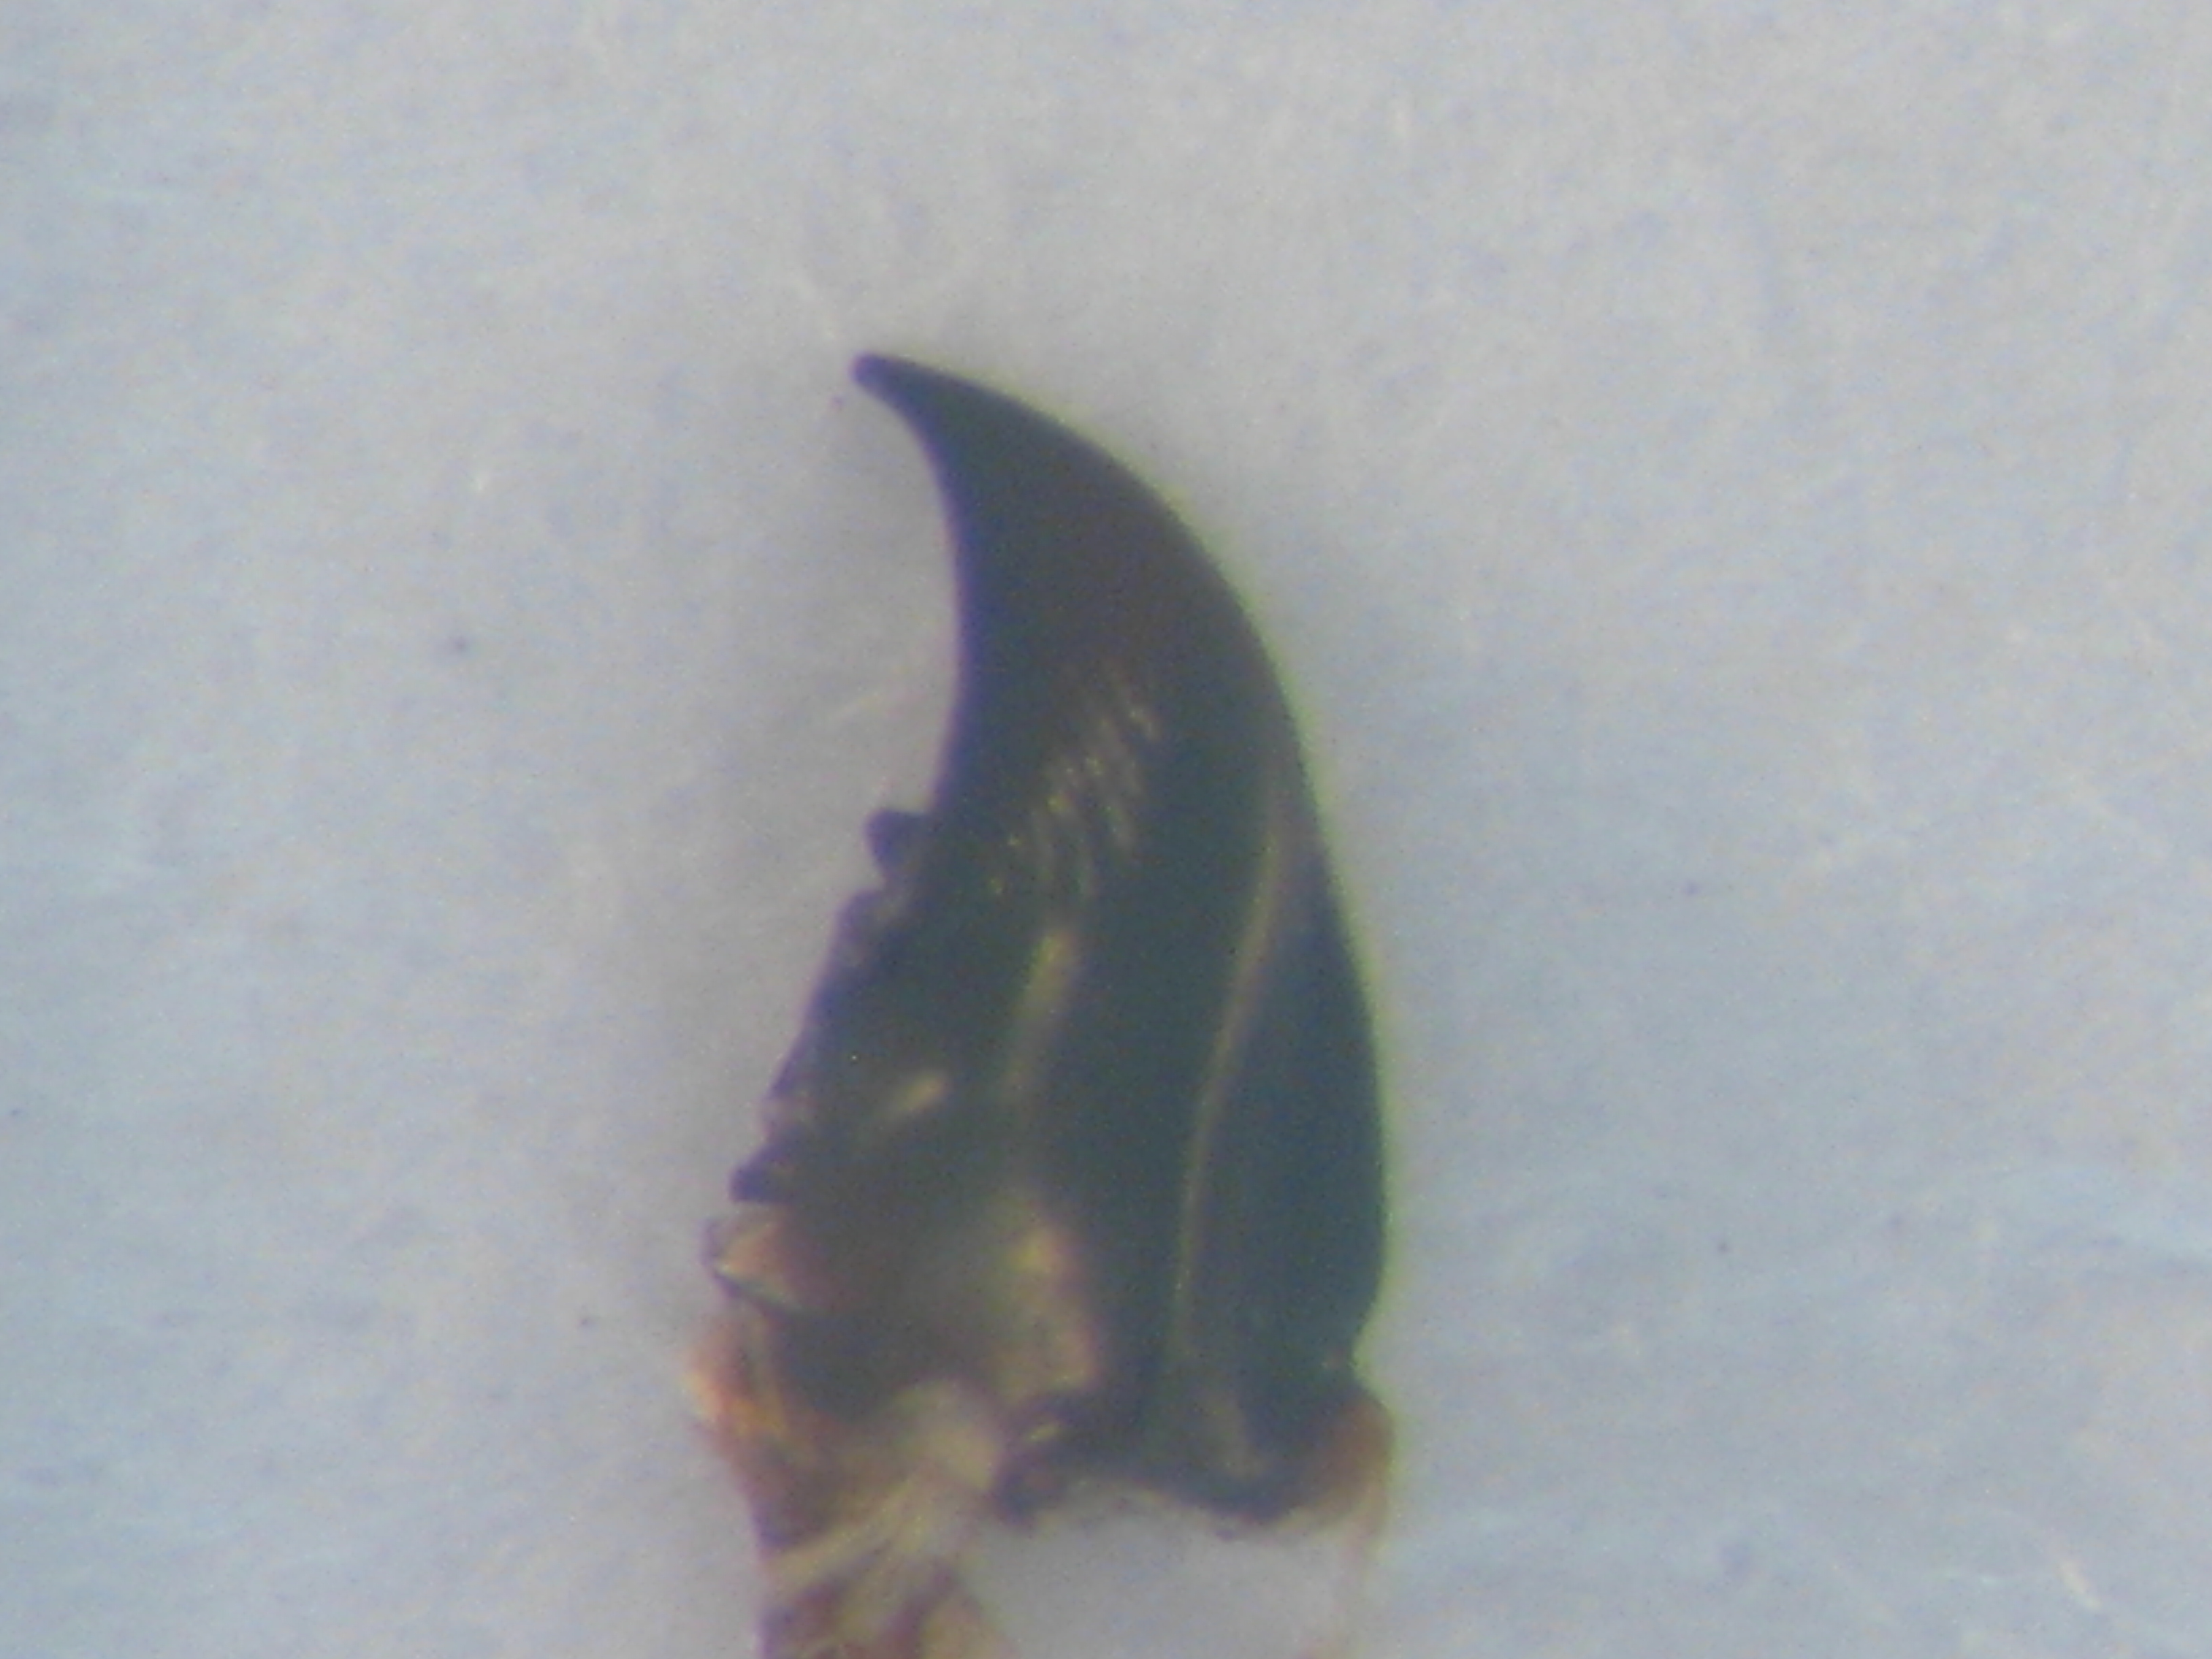
\includegraphics[width=0.2\textwidth]{./images/md32}}~~
\subfloat[Left mandible]
{\label{fig:example_112}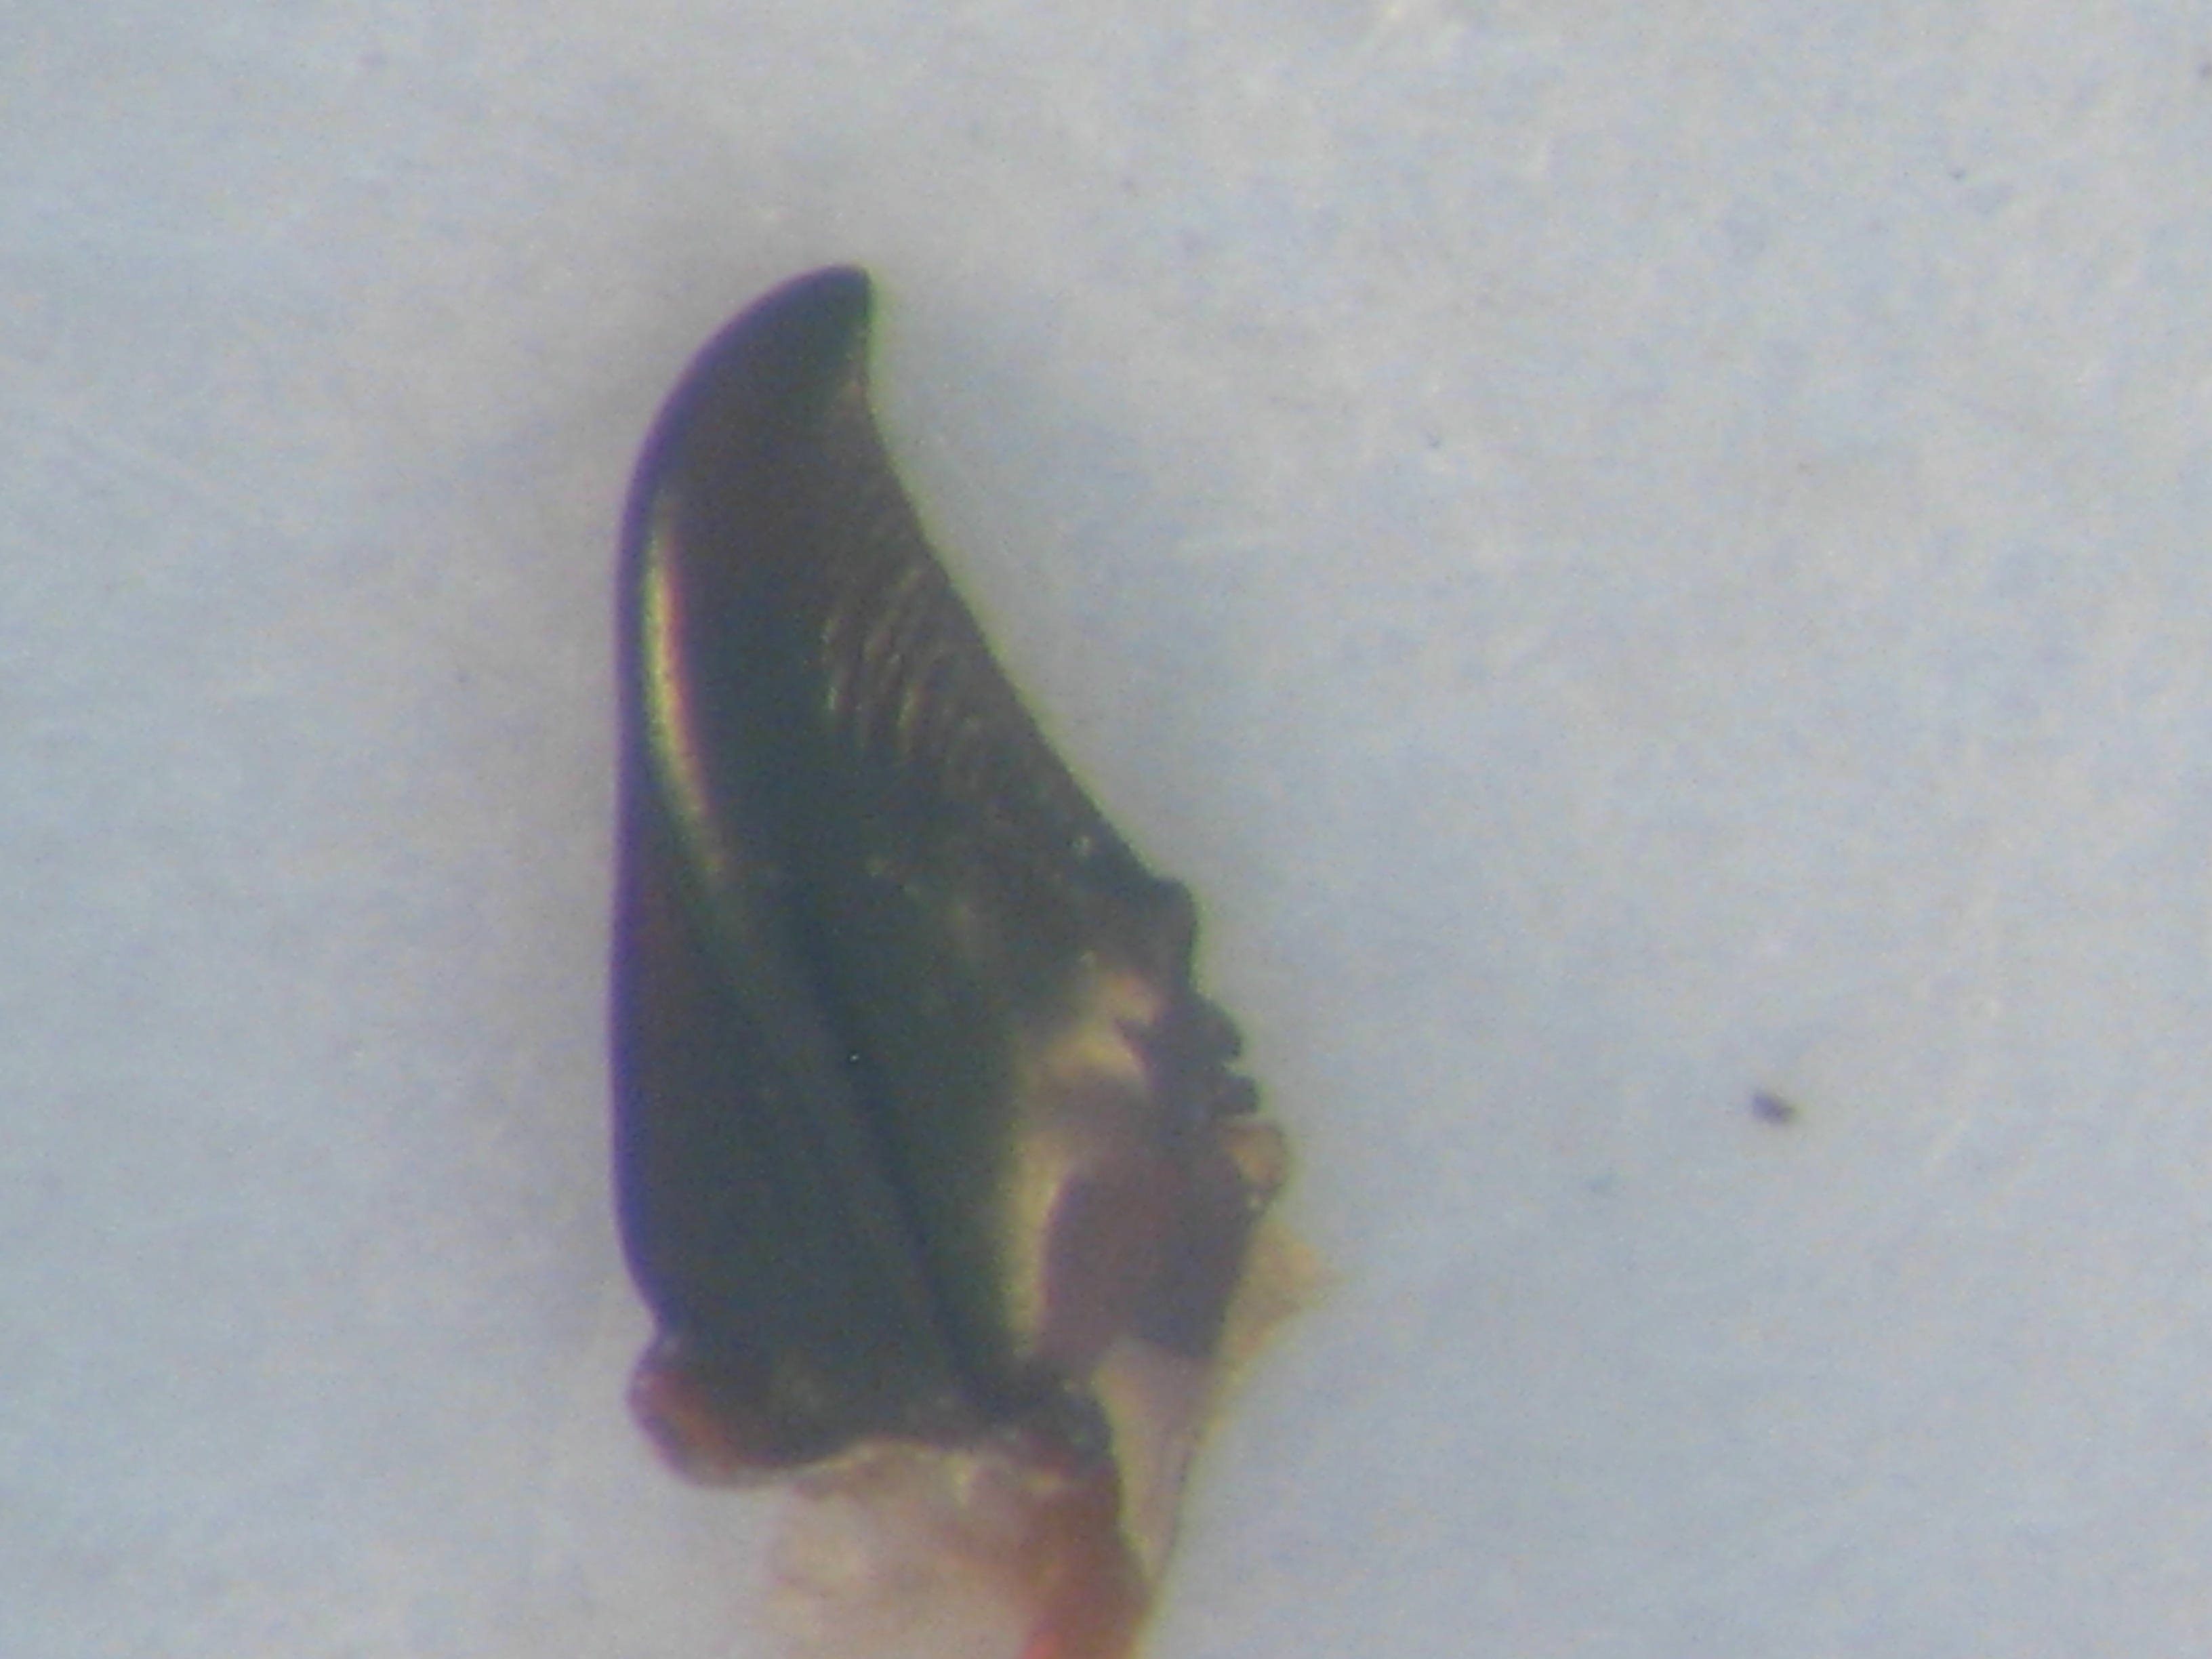
\includegraphics[width=0.2\textwidth]{./images/mg29}}
\caption{The mandibles of beetle}
\label{fig:figure_11}
\end{figure}~\\
In this paper, we focus on method to automatic identification of landmarks in digital images of the parts of beetle, specify are mandibles of beetle (figure \ref{fig:figure_11}). The method is constructed from four stages: a features extraction of mandible structure (segmentation stage), recording the features using pairwise geometric histogram (PGH), estimating the landmarks using Probabilistic Hough Transform (PHT) and refinement the estimated landmarks by cross-correlation.\\[0.3cm]
The proposed method extracts the features using the noise characteristics of image by analysing the histogram of image. The edges obtained are approximated by line segments and presented to PGH using geometric relationships between them. The shape correspondence is determined by comparing the PGHs of model and scene data. A PHT used to identify hypothesis landmarks location of the model on scene image. Finally, the hypothesis landmarks are performed by template matching.\\[0.3cm]
The data consists 291 digital images for each set of beetle's mandible (left mandible and right mandible (figure \ref{fig:figure_11})). This data set collected by biologist in INRA Rennes. Besides, the biologists also provide the set of manual landmarks for each mandible (they indicated by hand) (figure \ref{lm_example}).
\begin{figure}[h!]
\centering
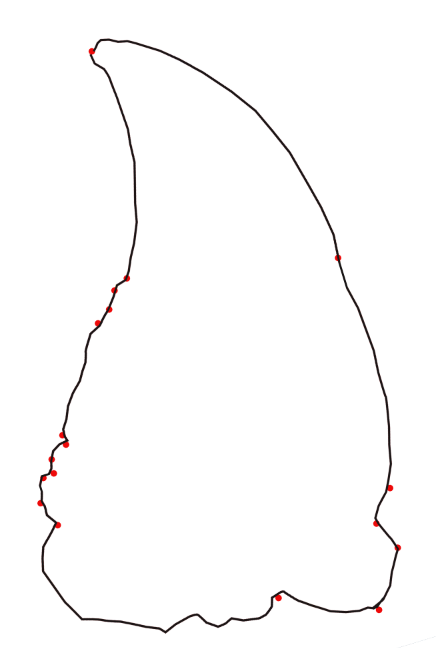
\includegraphics[width=0.15\textwidth]{./images/rshape}
\caption{Right mandible with the manual landmarks}
\label{lm_example}
\end{figure}
\section{Methods}
\subsection{Feature extraction}
The feature extraction stage extracts the information from the image that we interested in. By applying the suitable method to omit the noise, we can get the feature from the image. In this case, we analysis image's histogram (figure \ref{lm_hist}) to obtain the value for threshold segmentation. The threshold value is average value between two mean values of two regions on histogram (first region, begin from the histogram's begin to the median of histogram; second region is the rest of histogram).\\
\begin{figure}[h!]
\centering
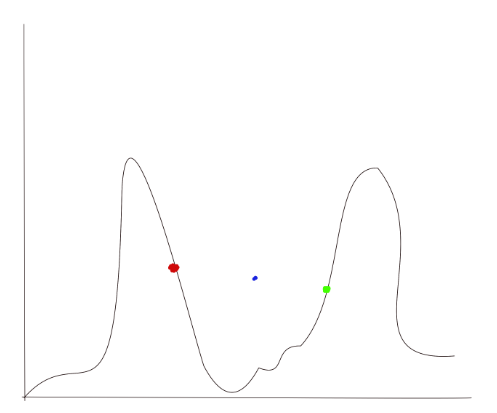
\includegraphics[width=0.4\textwidth]{./images/hist}
\caption{Histogram of image}
\label{lm_hist}
\end{figure}~\\
The Canny\cite{canny1986computational} algorithm is ideal for detection of edges, but need to analysis the topology\cite{suzuki1985topological} of image to retrieve the edges from image. The retrieved edges presented as a list of points. We need to present it to another kind of geometric to easy construct the PGH such as lines. The approximated lines obtained when we divide the edges. The process to break the edge into list of approximated lines as follows (this is a recursive algorithm\cite{thacker1995assessing}):
\begin{itemize}
	\item Create a line connected between two endpoints of the edge,
	\item For each point in the edge, we calculate the perpendicular distance from it to the line and keep the point where has the maximum distance (called maximum point),
	\item The edge is divided at the maximum point into two parts: one part begin from first endpoint to the maximum point, other one begin from the maximum point to the second endpoint of the edge,
	\item Continue with two new parts of the edges.
\end{itemize}
The algorithm stop when the edge can not break (actually, we decide that the algorithm stop when the maximum perpendicular less than 3 pixels (it enough small to create an approximated line)).
\subsection{Pairwise geometric histogram}
To determine the correspondence between the model and scene image, we present the approximated lines into PGH\cite{evans1993use} and calculate the similarity metric between the PGHs. The PGH is presented based on the geometric relationships between the lines, namely perpendicular distance and angle between the lines. This is a two dimensions matrix. It includes an axis presented for perpendicular distance and another axis presented for angle between the lines. Geometric relationships of all lines in the shape will presented on the same PGH. The steps to construct the PGH as follows:
\begin{itemize}
\item Create a PGH matrix,
\item Choose a reference line,
\item For each other lines in the shape,
	\begin{itemize}
		\item Calculating the perpendicular distance from two endpoints to the reference line,
		\item Computing the angle between the considered line and the reference line,
		\item Recording the perpendicular distance and angle into the matrix.
	\end{itemize}
\item Repeat step 2 (choose reference line) to all the lines in the shape considered as reference lines,
\item The algorithm stop when all lines of shape considered as reference line.
\end{itemize}
The PGH matching enables determine the similarity between the scene and model. The Bhattacharya\cite{palaniswamy2010automatic} similarity metric is used to compare the distribution (PGH) for the model and the scene data. It computes the degree of match between them and is expressed in the form of a dot product correlation of the PGHs (equation \ref{eq:1}).
\begin{center}
\begin{equation} \label{eq:1}
d_{Bhatt} (H_{i}H_{j}) = \sum\limits_{\theta}^{\pi}\sum\limits_{d}^{d_{max}}\sqrt{H_{i}(\theta,d)H_{j}(\theta,d)}
\end{equation}
\end{center}
\subsection{Probabilistic Hough Transform}
The PHT can be used to determined the presence and location of the model in the scene image. As well as determine the hypothesis of the model landmarks in the scene image. The applying PHT includes two steps: first, we find the pair of scene lines that similar with pair of the model lines (named training process); second, we estimate the model manual landmarks in the scene image(named estimate process).\\[0.2cm]
Training process includes the duration to construct the reference table for model image and process to find the similar pair of lines between model and scene image. The steps as follows:
\begin{itemize}
	\item Create the reference table,
		\begin{itemize}
			\item Choose an arbitrary point in the model,
			\item Create a table to record the information,
			\item For each pair of model lines, calculate the perpendicular distance and angle from each line to the point and save into the table.
		\end{itemize}
	\item Create an accumulator (a two dimension matrix (angle and perpendicular distance)),
	\item For each pair of scene lines, find the pair of model lines which correspondence about position, orientation and scale. Select the respective value in reference table,
	\item Increase the value in accumulator at respective position and keep the cell that have the maximum value.
\end{itemize}
The pair of scene lines that have the best vote in the accumulator are the pair of lines chosen. From the pair of scene line, extending the perpendicular distance at right position, we can estimated the reference point in the scene image.\\[0.3cm]
The estimated landmarks in the scene obtained by calculating the relatedness between the model's reference point and the model's landmarks. Besides, we also record the difference angle between model image and the scene image. 
\begin{figure}[h!]
\centering
\subfloat[The model image]
{\label{fig:example_121}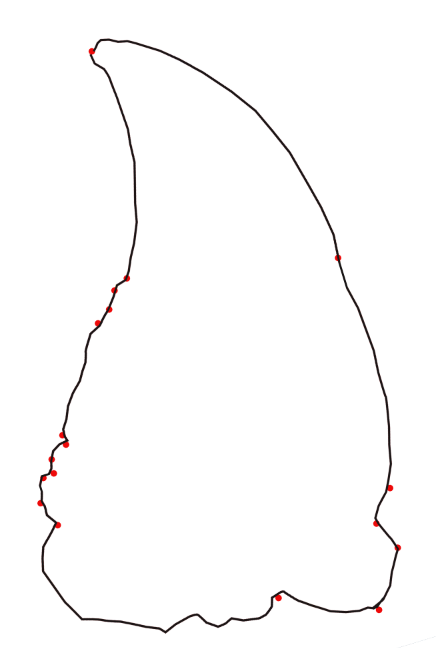
\includegraphics[width=0.2\textwidth]{./images/rshape}}~~
\subfloat[The scene image]
{\label{fig:example_122}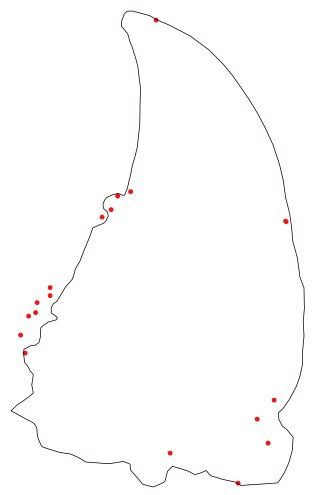
\includegraphics[width=0.2\textwidth]{./images/training}}
\caption{The estimated landmarks by PHT}
\label{fig:figure_12}
\end{figure}
\subsection{Template matching}
The template matching is process to verify the estimated landmarks in PHG stage. And cross-correlation is hired for this work. By sliding the template on image by each pixel, cross-correlation will detect the best similar between model and scene image. The progress of template matching as follows:
\begin{itemize}
\item Rotate the scene image (the angle has indicated by PHT),
\item Create a bounding box around a model manual landmark (in model image),
\item Create a bounding box around a estimated landmark (in scene image),
\item Apply cross-correlation between two bounding boxes.
\end{itemize}
The template matching finishes when all estimated landmarks are refined.
\begin{figure}[h!]
\centering
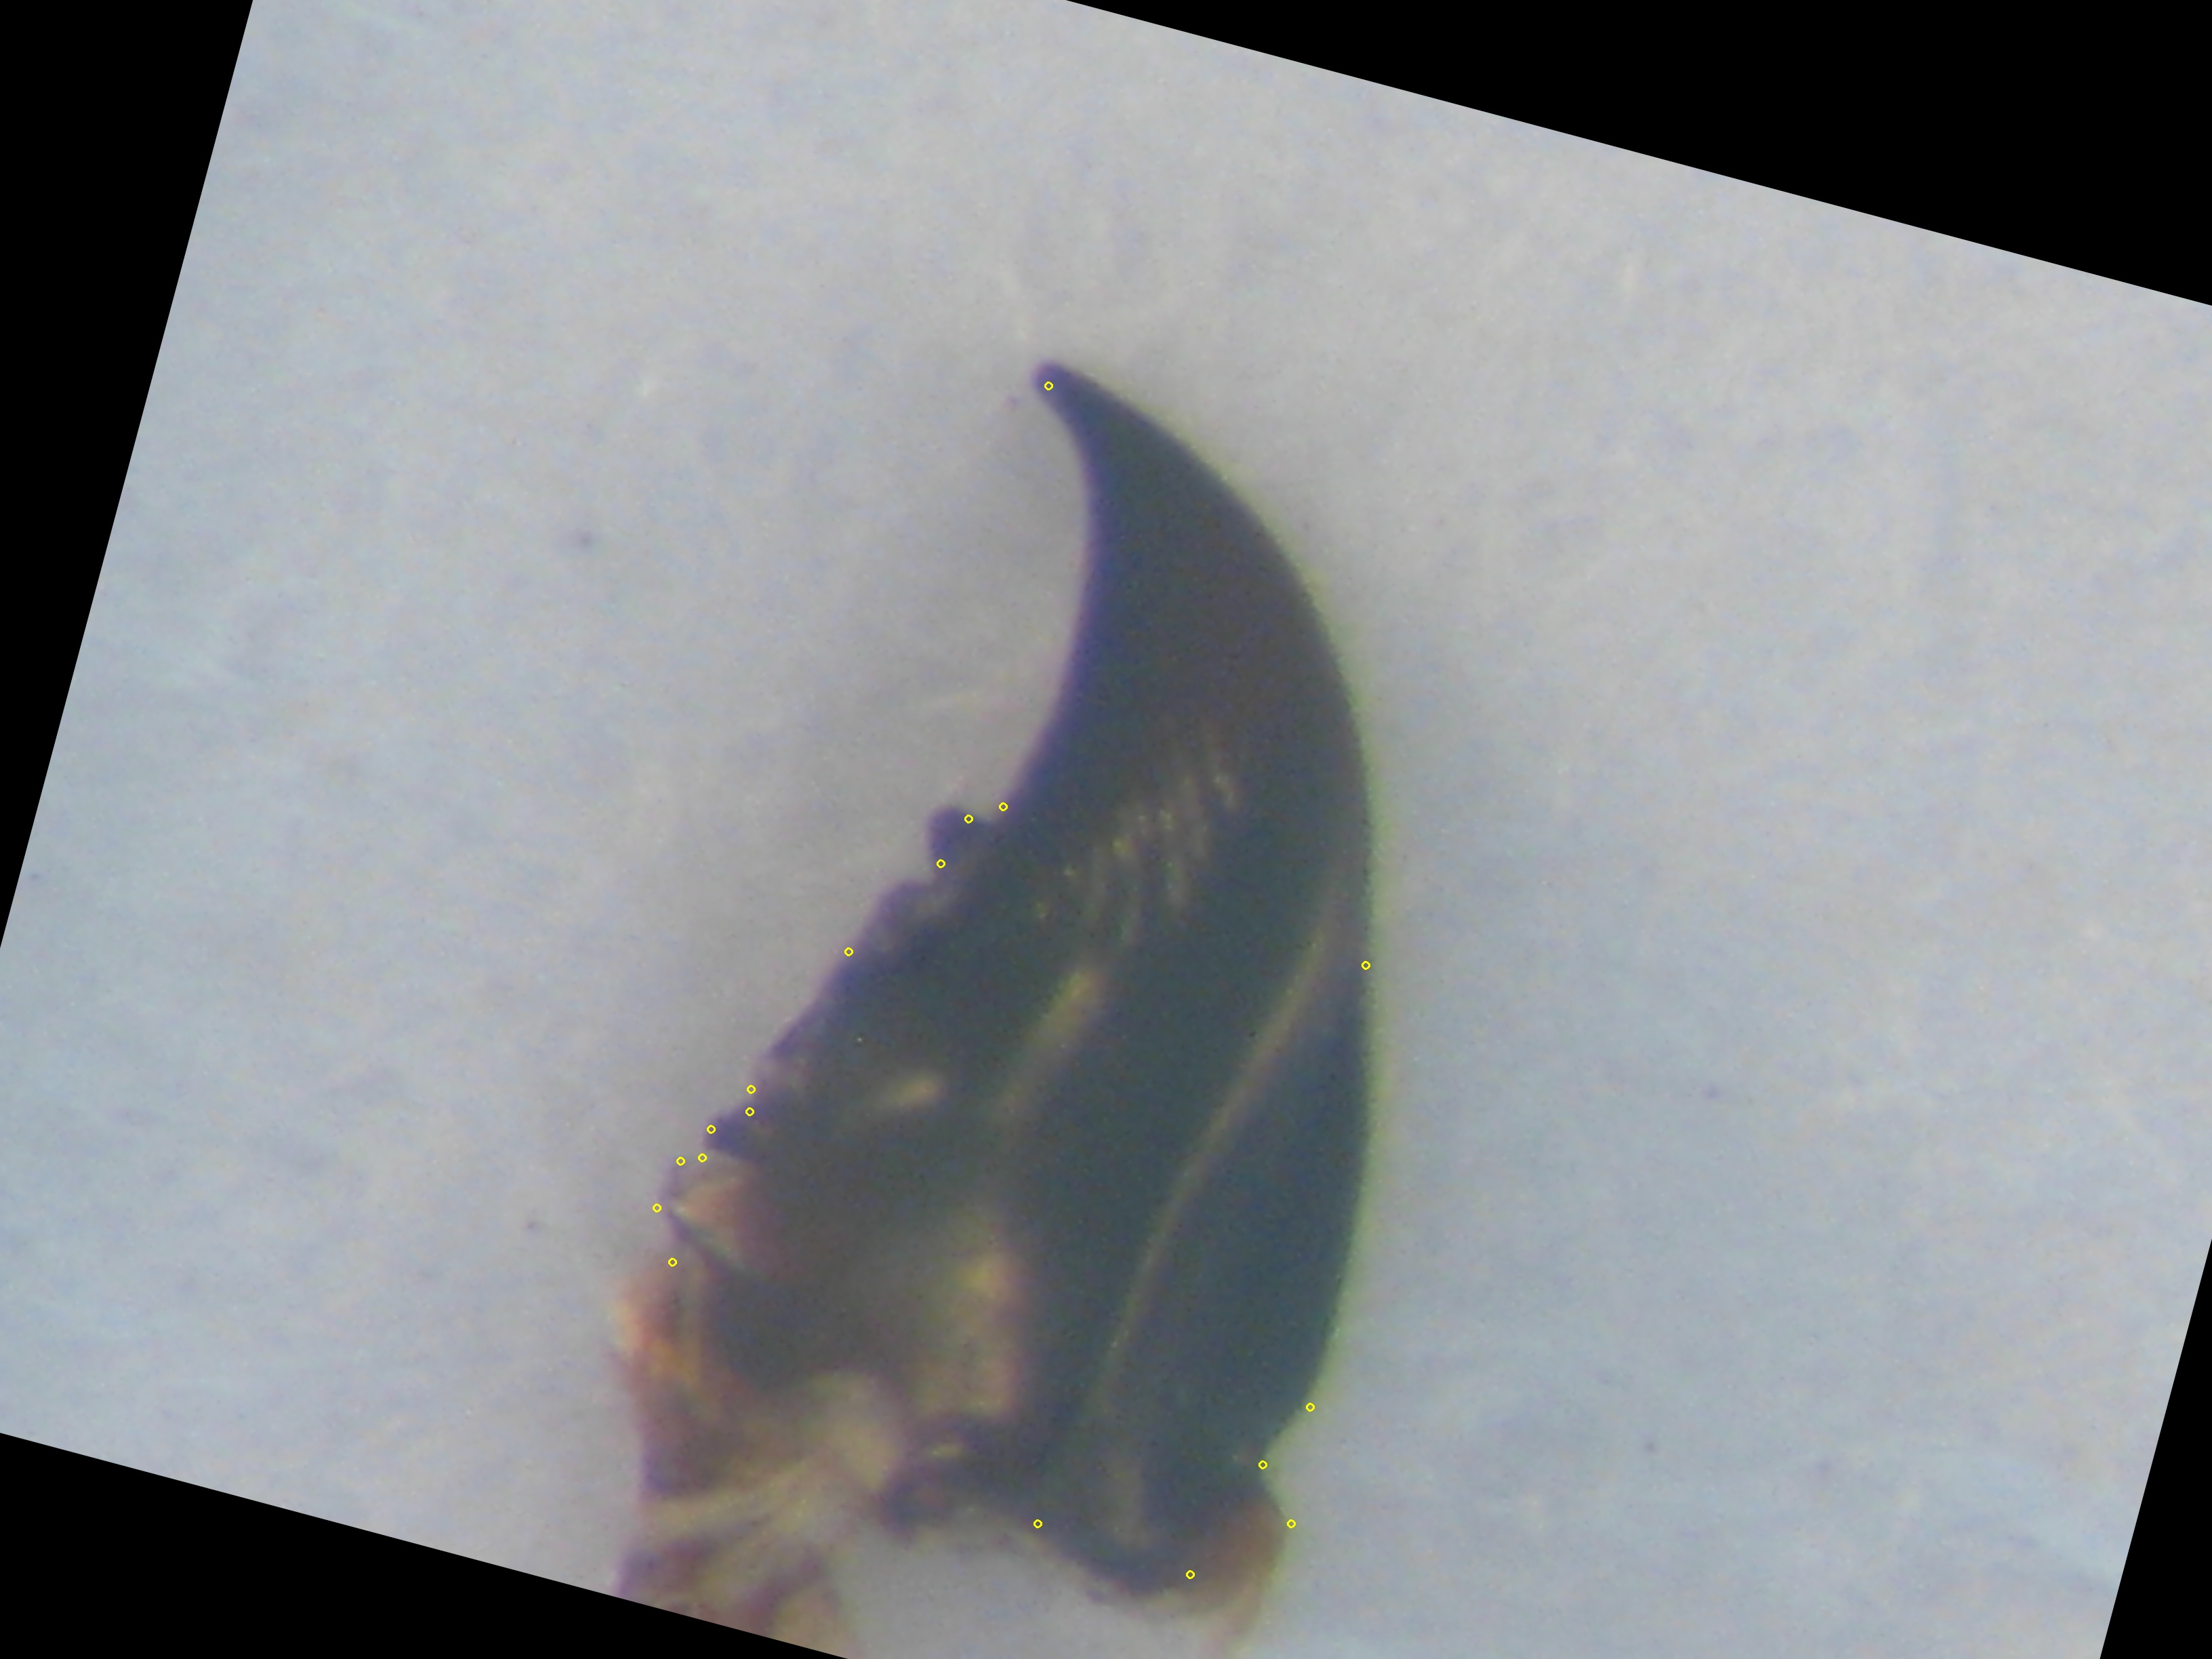
\includegraphics[width=0.4\textwidth]{./images/est32}
\caption{Automated landmarks in scene image after refining}
\label{lm_hist}
\end{figure}~\\
\section{Experiment and result}
\section{Conclusion}
\section{References}
\bibliographystyle{plain}
\bibliography{./includes/references}
\end{document}